\chapter{Datenverarbeitung}
\label{ch:data_processing}

\section{Verarbeitung Apache Spark\texttrademark}
Der physikalische Aufbau wurde bereits im Grundlagenkapitel zu Apach Spark behandelt (siehe Kapitel \ref{sec:theory_spark}). In diesem Kapitel sollen primär die Algorithmen und die Verarbeitung der Daten aus logischer Sicht betrachtet.\\ 

\noindent
Bei Apache Spark gibt es seit der Version 2.0.0 diverse APIs, wie Daten geladen werden können. Es besteht die Möglichkeit Daten mithilfe von Resilient Distributed Datasets (RDDs) zu laden und zu verarbeiten. Aufbauend auf diesen RDDs können, die Daten gemappt, gefilter oder aggregiert werden. Dies Möglichkeit gibt es schon immer in Apache Spark. Seit der Version 2.0.0 gibt es nun auch DataFrames und DataSets (TODO: gibt es beides erst seit v2.0?). Diese Datenstrukturen beschreiben eher eine Schnittstelle aus Sicht von Tabellen. Die Implementierung dieser Typen baut wieder auf den RDDs auf. Doch welche Strukturen eignen sich für die Anwendungsfälle in dieser Thesis? \\

\noindent
DataFrames und DateSets sind optimiert für strukturierte und semi-strukturierte Daten. Diese Daten lassen sich beispielsweise in Tabellenstrukturen einlesen und verarbeiten. Es gibt High-Level Operationen auf diesen Tabellen, welche dem klassischen SQL Syntax sehr nahe kommen?! Apache Spark selbst kann bei der Nutzung von DataFrames und DataSets viele Optimierungen bei der Ausführung und Verarbeitung durchführen. Andererseits sind diese Strukturen ungeeignet bei unstrukturierten Daten, wie beispielsweise Multimediadateien und eben auch beliebigen Dateien.\cite[S. 66 ff.]{data_processing_spark2}\\

\noindent
Wie beim Datenimport schon beschrieben, sind die Metadaten der analysierten Datenträger strukturiert beziehungsweise semi-strukturiert in HBASE abgespeichert. Prinzipiell wäre es also möglich, auch mit Datasets und Dateframes auf diese Daten zuzugreifen. Letztlich kommt es auch auf die Anbindung zwischen Apache Spark und Apache HBASE an. Hierbei gibt es primär zwei unterschiedliche Connectoren\footnote{Bei Apache Spark sind Connectoren eine Art von Java-Bibliotheken, welche es ermöglichen im Apache Spark Ausführungskontext auf andere Systeme, wie beispielsweise Datenbanken oder Dateisysteme, zuzugreifen.}. Der \textit{Hortonworks SHC} Connector ermöglicht die Interaktion mit Daten in HBASE und nutzt dafür die DataFrame/DataSet Datenstrukturen.\footnote{Siehe \url{https://github.com/hortonworks-spark/shc}, Stand: 15.6.2018.} 
Also Pendant auf Basis von RDDs existiert ein weiterer \textit{hbase-spark} Connector. Letzterer wird im Rahmen dieser Thesis genutzt, um Daten von HBASE zu lesen und zu schreiben.\footnote{Siehe \url{https://github.com/apache/hbase/tree/master/hbase-spark}, Stand: 15.6.2018 und deren Nutzung im Projekt \textit{foam-processing-spark} unter \url{https://github.com/jobusam/foam-processing-spark}, Stand: 16.5.2018.}

\subsection{Praxisbeispiele und deren Optimierungen}
Gerade bei der Verarbeitung großer Datenmengen und unter Berücksichtigung des Prinzips der Datenlokalität existieren einige Fallstricke und Hürden bei der Implementierung der Datenverarbeitung. Im Hadoop-Umfeld und bei der Entwicklung im Spark-Context geht es nicht nur um die Art und Weise, wie die Algorithmen auf die Daten angewendet werden, sondern in erster Linie auch immer darum \textbf{wo} die einzelnen Programmteile ausgeführt werden. 
Der Entwickler sollte immer wissen, in welchem Verarbeitungskontext er sich befindet. Zu dieser Problematik werden in diesem Kapitel einige Beispiele herausgegriffen, welche während der Bearbeitung dieser Thesis aufgetreten sind.\\

\noindent
\subsubsection*{Weniger ist mehr TODO}
Ungenutzte Daten so früh wie möglich aus der Verarbeitung rausnehmen. Siehe
Problematik beim HBASE-Spark Connector. Entweder ich mache einen Full-Table Scan und fodere
alle Daten an, um sie später im Spark-Executor auszuführen, oder ich versuche schon beim Zugriff der Daten in den Region-Server mit ColumnFamilies und Filter-Operationen nur die Daten anzufordern, welche auch wirklich benötigt werden. 
\subsubsection*{Caching - Performanz vs. Ressourcen TODO}
Hashing-Problem. Ist es geschickter Daten zu Cachen anstatt sie zweifach anzufordern?
Funktioniert Caching überhaupt mit nicht serializierbaren Daten?
\subsubsection*{Faulheit ist der Schlüssel zum Erfolg TODO}
Lazy-Loading und Ausführung bei RDDs

\subsubsection*{Teile und Herrsche TODO}
Balancing and Repartitionieren. Aufteilung der Last zu gleichen Teilen!
Gerade beim Ausprobieren und Testen ist es einfach, die Resultate eines RDDs nach der Datenverarbeitung über eine Konsole auszugeben. Doch hierbei muss genau überlegt werden, wie diese Resultate ausgegeben werden (siehe Listing \ref{lst:spark_rdd_collect}). In der ersten Variante wird auf dem RDD die Methode collect() aufgerufen und die daraus erhaltene Liste von Objekten wird über ein Logger-Objekt in das Log-File dieser Ausführung geschrieben.\\
Auf der ersten Blick ist aber nicht ersichtlich, was diese Methode wirklich bewirkt. Wie bereits in Kapitel \ref{sec:theory_spark} (TODO: check reference) beschrieben, wird bei der Ausführung einer Spark-Anwendung ein sogenannter Spark-Driver gestartet. Dieser wiederum fordert eine gewisse Anzahl von Exekutoren an, die die eigentlich Datenverarbeitung übernehmen (Master-Slave-Prinzip). Hierbei laufen die Executoren auf einzelnen Knoten innerhalb des Clusters. In dem Moment, in welchem die collect()-Methode auf einem RDD ausgeführt wird, werden die Daten des RDDs \textit{eingesammelt}. Dies bedeutet, dass die Daten des RDDs, welche vorher verteilt auf allen Executoren im Arbeitsspeicher geladen wurden, nun jetzt an den Spark-Driver geschickt werden. Dieser sammelt sozusagen die Ergebnisse der Executoren ein. Diese Mechanismus ist an sich nicht problematisch und funktioniert auch gerade beim Testen mit kleinen Datenmengen. Bei großen RDDs hingegen, werden auch wieder alle Daten an der Driver geschickt und in den meisten Fällen wird dies den begrenzten Arbeitsspeicher des Drivers überfordern. Die Applikation wird mit einer OutOfMemoryException??? beendet!.\\

\noindent
Daher ist es sinnvoll auch schon beim Testen mit kleinen RDDs vorzugsweise die take()-Methode zu nutzen. Diese tut das gleiche wie, die collect()-Methode mit dem Zusatz, dass sie nur ein bestimmte Anzahl von Einträgen sammelt. Dadurch wird selbst bei größeren RDDs der Speicher nicht ausgehen. 


\begin{lstlisting}[label={lst:spark_rdd_collect},caption= Spark Java RDD collect()-Methode ,captionpos=b,frame=single,style=customshell]

HbaseReader hbr = new HbaseReader(jsc, hbaseConfigFile);
JavaRDD<Metadata> forensicMetadata = hbr.getForensicMetadata();

# use collect() method
forensicMetadata.collect().stream()
	.forEach(m -> LOGGER.info("Entry = .", m));

# use take(int amount) method	
forensicMetadata.take(10).stream()
	.forEach(m -> LOGGER.info("Entry = .", m));	
\end{lstlisting}


\section{Anwendungsfälle der Datenverarbeitung}
\subsection{Hashsummen ermitteln}
Die Hashsummenermittlung erfolgt auf Basis von SHA-512, da kryptografisch sicher (siehe Hacking-Buch)\\

\noindent
NIST Hash Dataset von SW -> known good files\cite[S. 36]{digital_forensics}
\subsection{Dateityp erkennen mit Apache Tika}

\subsection{Dateien indizieren}
Ein weitere Anwendungsfall ist die Indizierung von Texten und Wörtern, welche aus den einzelnen Dateien extrahiert wurden.\\

\noindent
Der Grund für eine Indizierung dieser Inhalte ist eine schnellere Suche nach beliebigen Wörtern, als bei der reinen Suche in HBASE. Zur Indizierung existieren zwei bekannte Projekt. Diese sind einerseits \textit{Apache Solr} und andererseits \textit{Elasticsearch}. Bei bauen wiederum auf das \textit{Apache Lucene}-Projekt auf. Apache Solr ist ein Open-Source Projekt unter dem Dach der Apache Foundation. Wohingegen Elasticsearch auch als Open-Source Projekt entwickelt wird, jedoch primär von der kommerziellen Firma \textit{Elastic???} verwaltet wird. Diese bietet gerade Zusatzpakete und Support gegen Bezahlung an.
Siehe auch \cite[S.7]{solr_search}
\subsubsection{Apache Solr}
Spark-Connector von Databracks vorhanden. Der Connector selbst bietet aber vorzugsweise lesenden Zugriff.

\noindent
Abbildung \ref{fig:hbase_solr_indexing} stellt die physikalische Aufteilung mit dem hbase-indexer projekt

\begin{figure}[ht]
  \centering
  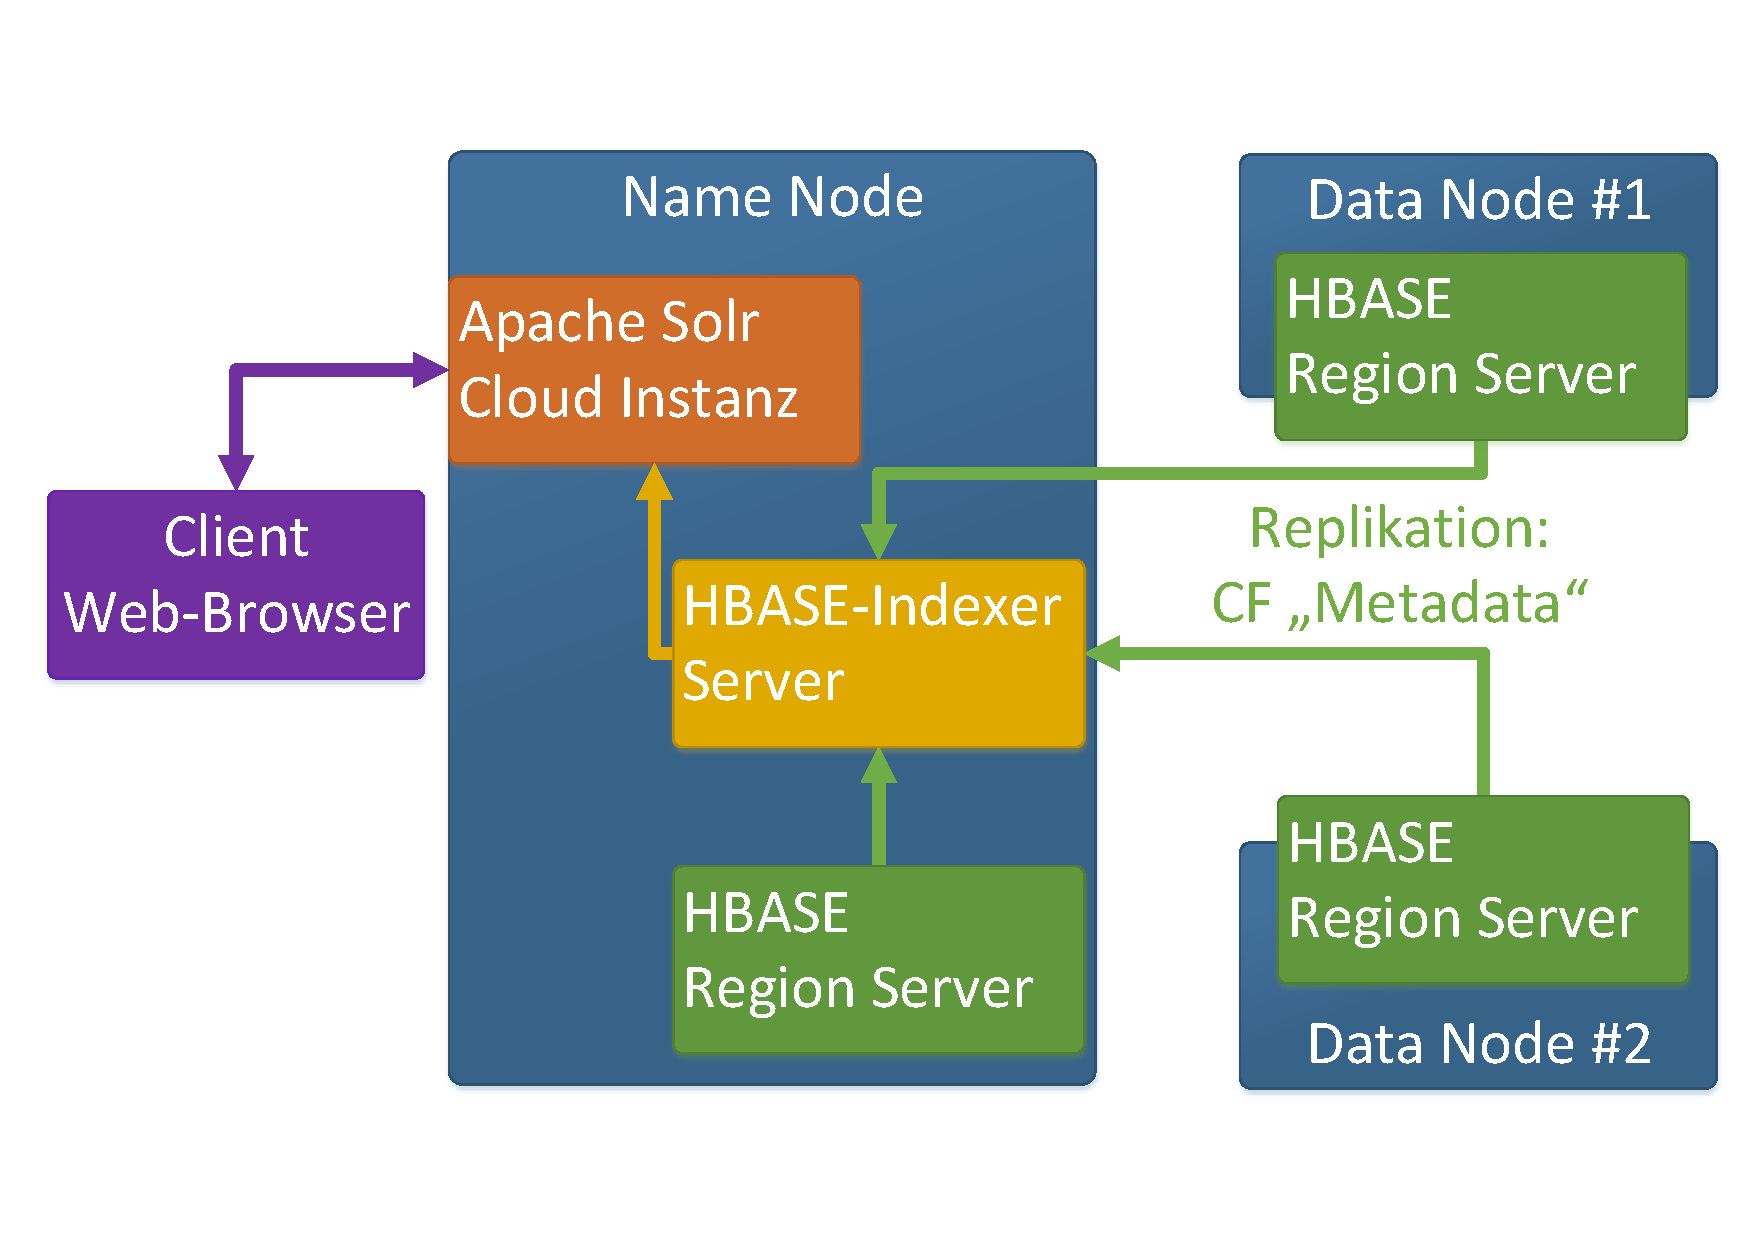
\includegraphics[width=\textwidth]{./resource/hbase_solr_indexierung.pdf}
  \caption{Indexierung von Daten aus HBASE in Solr}
  \label{fig:hbase_solr_indexing}
\end{figure}

\subsubsection{Elasticsearch}
Spark-Connector auf RDD-Basis vorhanden. Kerberos-Sicherung nur über X-Pack gegen Geld vorhanden. Rack-Awareness und Verteilung nicht klar. Elasticsearch baut eigene Infrastruktur auf. Nicht über Ambari steuerbar.